\documentclass[11pt]{beamer}
\usepackage[utf8]{inputenc}
\usepackage[italian]{babel}
\usepackage{amsmath}
\usepackage{amsfonts}
\usepackage{amssymb}
\usepackage{graphicx}
\pdfmapfile{+sansmathaccent.map}
\usetheme{metropolis}
\makeatletter
\begin{document}	
	\author{Michele De Vita}
	\title{Sviluppo di un'applicazione Android per il posizionamento indoor}
	%\subtitle{}
	%\logo{}
	%\institute{}
	\date{14 luglio 2017}
	%\subject{}
	%\setbeamercovered{transparent}
	%\setbeamertemplate{navigation symbols}{}
	\begin{frame}[plain]
		\maketitle
	\end{frame}
	
	\begin{frame}{Cos'\`e il posizionamento \textit{indoor}?}
		\begin{itemize}
			\item Una delle tecniche pi\`u usate per il posizionamento \textit{outdoor}, la triangolazione GPS, non si pu\`o usare all'interno degli edifici a causa delle distorsioni provocate da muri e tetti.
			\begin{figure}
				\centering
				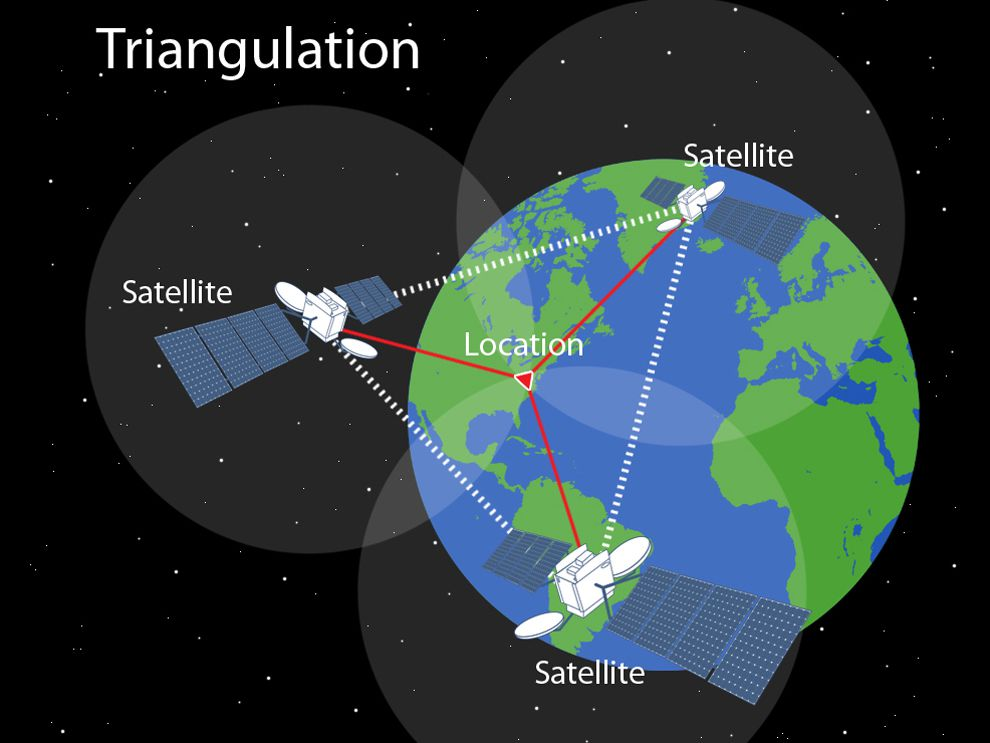
\includegraphics[width=0.7\linewidth]{img/gps_triangulation}
			\end{figure}
		\item Perci\`o si ricorre a tecniche alternative per il posizionamento \textit{outdoor}
		\end{itemize}
	\end{frame}
	\begin{frame}{Cos'\`e il posizionamento \textit{indoor}?}
		\begin{itemize}
			\item Molte aziende stanno investendo in questo settore ed anche in ambito accademico escono pubblicazioni scientifiche.
			\item Adesso vediamo alcune tecniche di posizionamento \textit{indoor}:
				\begin{itemize}
					\item \textit{Wi-Fi}
					\item \textit{BLE Beacons}
				\end{itemize}
			\item Durante il tirocinio mi sono occupato del posizionamento \textit{indoor} sfruttando la distorsione del campo magnetico terrestre.
		\end{itemize}
	\end{frame}
	\begin{frame}{Alcuni casi d'uso del posizionamento \textit{indoor}}
		\begin{itemize}
			\item Nel museo: l'applicazione ufficiale apre un \textit{pop-up} in automatico che ci mostra informazioni aggiuntive sull'opera che stiamo visualizzando
			\item In aeroporto : ci potrebbe indicare la strada da percorrere per raggiungere il \textit{gate} 
		\end{itemize}
	\end{frame}
	\begin{frame}{Onde magnetiche: cosa sono?}
		\begin{itemize}
			\item \`E un vettore composto da un verso, direzione ed intensit\`a
			\item L'unita di misura \`e il $\mu$T (micro Tesla)
			\item I valori del vettore variano in base ai materiali presenti intorno
			\item Durante la localizzazione \textit{indoor} sfruttiamo le onde generate dalla Terra e la distorsione generata dagli oggetti all'interno dell'edificio
		\end{itemize}
		\begin{figure}
			\centering
			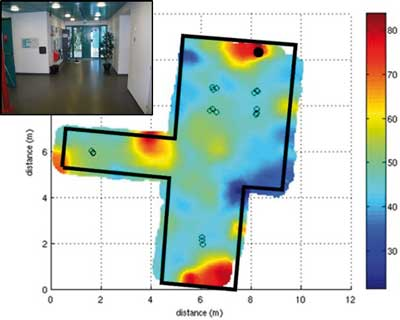
\includegraphics[width=0.5\linewidth]{img/magnetic_field_map}
		\end{figure}
	\end{frame}
	\begin{frame}{\textit{Smartphone} ed onde magnetiche}
		\begin{itemize}
			\item Su ogni \textit{smartphone} \`e presente il magnetometro, un sensore capace di catturare il campo magnetico.
			\item Quando si registrano le onde magnetiche su \textit{Android}, viene restituita una sequenza di 3 elementi rappresentante l'intensit\`a del campo magnetico lungo i 3 assi mostrati qua sotto.
			\begin{figure}
				\centering
				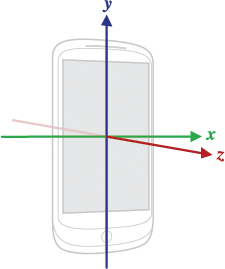
\includegraphics[width=0.4\linewidth]{img/axis_magnetic_field}
			\end{figure}
		\end{itemize}
	\end{frame}
	\begin{frame}{Elaborazione e classificazione dei dati}
		\begin{itemize}
			\item Una volta raccolti i dati, vanno elaborati per rendere pi\`u efficace la classificazione.
			\item Ci sono molte tecniche che possiamo usare, pi\`u efficaci o meno in base al tipo di dato trattato.
			\item Le tecniche pi\`u usate possiamo riassumerle in queste 3 macro categorie:
				\begin{itemize}
					\item Scalatura dei valori
					\item Estrazione di attributi
					\item Selezione di attributi
				\end{itemize}
		\end{itemize}
	\end{frame}
	\begin{frame}{Apprendimento automatico}
		\begin{itemize}
		\item Branca dell'IA che conferisce al calcolatore l'abilit\`a di apprendere senza essere esplicitamente programmati.
		\item Tipi di apprendimento:
			\begin{itemize}
				\item Supervisionato
				\item Non supervisionato
				\item Rinforzo
			\end{itemize}
		\item Durante il tirocinio si \`e utilizzato l'apprendimento supervisionato con output un valore discreto (classificazione)
		\end{itemize}
	\end{frame}
	\begin{frame}{Un esempio di classificazione}
		\begin{figure}
			\centering
			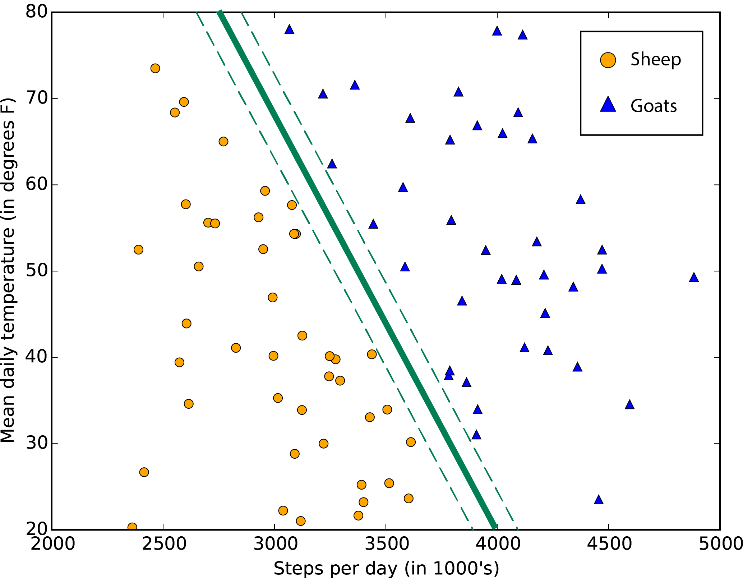
\includegraphics[width=0.7\linewidth]{img/supervised_learning_example}
		\end{figure}
	\end{frame}
	\begin{frame}{Classificazione e regressione a confronto}
		\begin{figure}
			\centering
			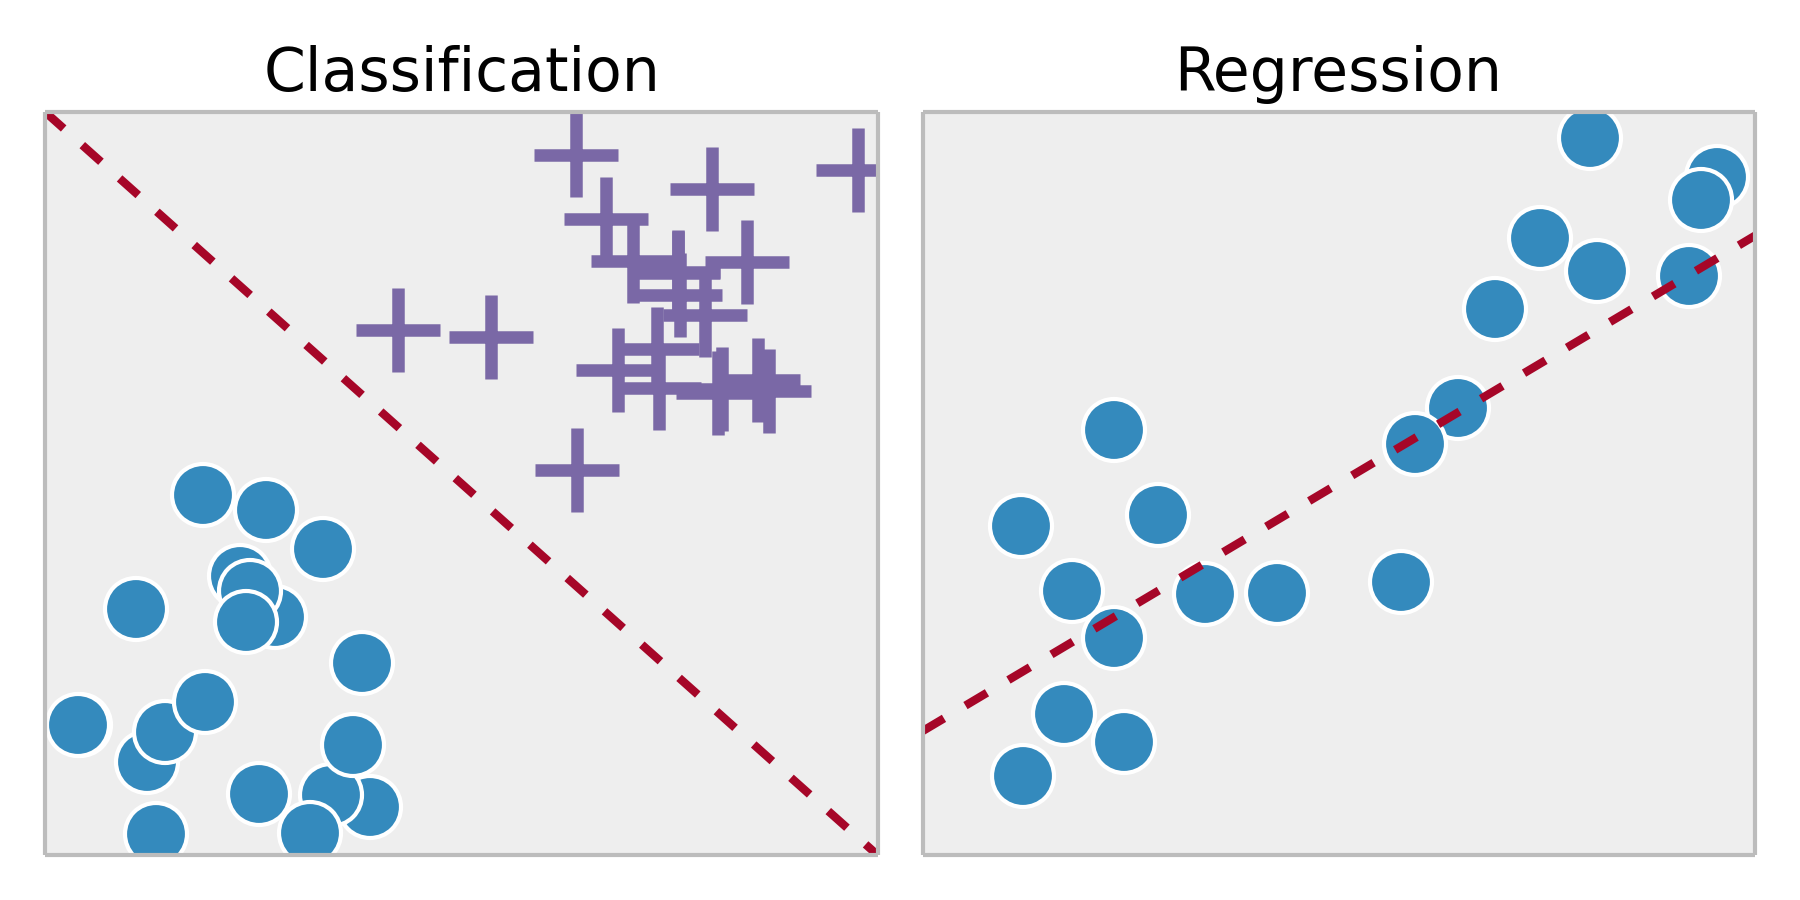
\includegraphics[width=0.7\linewidth]{img/Classification_Regression}
		\end{figure}	
	\end{frame}
	\begin{frame}{Alcune nozioni sull'apprendimento automatico}
		\begin{itemize}
			\item Rumore: dati contenenti valori anomali od errori.
			\item \textit{Overfitting}: il modello si \`e adattato troppo ai nostri dati.
			\item \textit{Underfitting}: problema opposto al precedente: il modello ha imparato troppo poco.
			\item Parametri: valori del modello stabiliti internamente.
			\item Iper-parametri: valori stabiliti dal suo creatore.
			\item Insieme di addestramento: sottoinsieme del \textit{dataset} di partenza su cui il modello apprende.
			\item Insieme di validazione: sottoinsieme usato per cercare i migliori iper-parametri.
			\item Insieme di test: sottoinsieme usato per verificare l'efficacia del modello.
		\end{itemize}
	\end{frame}
	\begin{frame}{Overfitting ed underfitting}
		\begin{center}
			\centering
			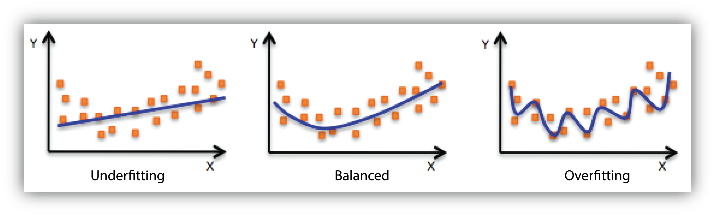
\includegraphics[width=1.1\linewidth]{img/underfittingoverfitting}
		\end{center}
	\end{frame}
	\begin{frame}{\textit{Cross-validation}}
		\begin{itemize}
			\item Invece di avere un insieme di addestramento e validazione, si divide l'insieme d'addestramento in n parti. A turno ciascuna parte svolge il ruolo di insieme di validazione mentre il resto d'addestramento.
			\item Molto utile per dataset piccoli
		\end{itemize}
		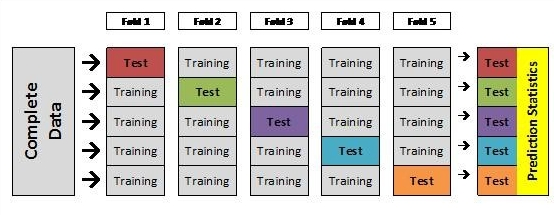
\includegraphics[width=0.7\linewidth]{img/crossvalidation}
	\end{frame}
	\begin{frame}{Valutazione delle prestazioni e metriche}
		\begin{itemize}
			\item Per valutare la potenza del classificatore si effettuano predizioni sull'insieme di test e si utilizza una metrica per quantificarla.
			\item Durante il tirocinio l'obbiettivo \`e stato quello di massimizzare l'accuratezza (predizioni corrette su grandezza dell'insieme di test)
			\item Un'alta accuratezza non \`e sempre sinonimo di un buon modello.
		\end{itemize}
	\end{frame}
	\begin{frame}{Classificatori usati per la predizione della posizione}
		\begin{itemize}
			\item Knn
			\item Alberi di decisioni
		\end{itemize}
	\end{frame}
	\begin{frame}{Knn}
		\begin{itemize}
			\item Non ha una fase di addestramento
			\item La predizione si svolge nel seguente modo:
				\begin{enumerate}
					\item Trova i k elementi che minimizzano la distanza dalla nuova istanza.
					\item La classe pi\`u frequente tra i vicini diventa quella assegnata ai nuovi attributi.
					\item L'unico iper-parametro \`e k.
				\end{enumerate}
			\item La distanza si pu\`o definire in vari modi: useremo la distanza euclidea
		\end{itemize}
	\end{frame}
	\begin{frame}{Knn}
		\begin{center}
			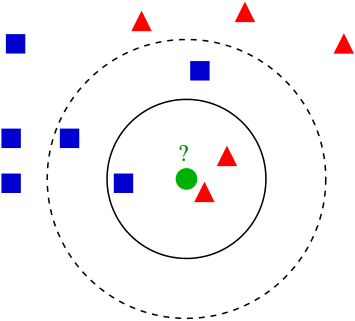
\includegraphics[width=0.7\linewidth]{img/knn_example}
		\end{center}
	\end{frame}
	\begin{frame}{Alberi di decisione}
		\begin{itemize}
			\item Costruzione dell'albero (Addestramento): dagli esempi vengono costruiti i nodi interni in base all'attributo che li suddivide meglio (minimizza il decremento d'impurit\`a). La costruzione di un albero si ferma in base a vari criteri, impostabili tramite iper-parametri. 
			\item Predizione: scorrere l'albero in base ai valori presenti nell'istanza da classificare, per poi arrivare in una foglia, che diventer\`a la nuova classe.
		\end{itemize}
	\end{frame}
	\begin{frame}{Alberi di decisione}
		\begin{center}
			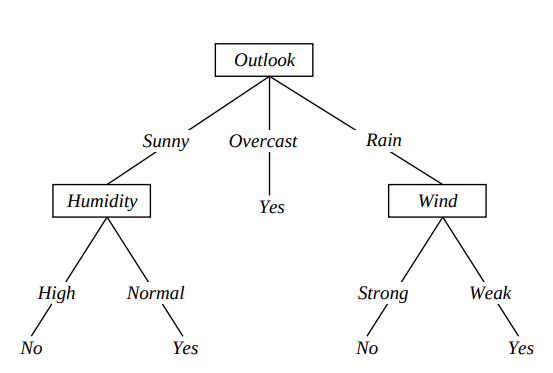
\includegraphics[width=0.7\linewidth]{img/decision_tree_tree_tennis}
		\end{center}
	\end{frame}
	\begin{frame}{Applicazione}
		\begin{itemize}
			\item Sviluppata su \textit{Android} API 24 (Lollipop) mantenendo una retrocompatabilit\`a con le versioni precedenti
		\end{itemize}
		\begin{align*}
    	 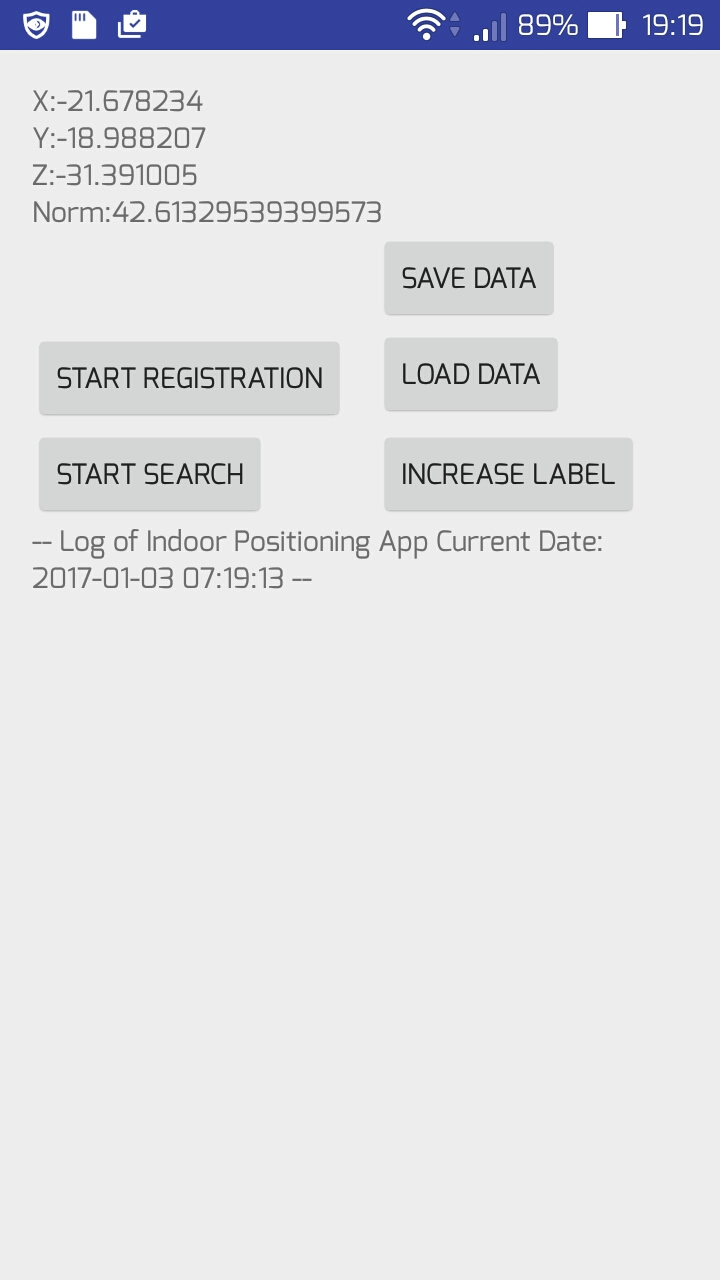
\includegraphics[width=0.3\linewidth]{img/app_screen} \,\,\,			
	     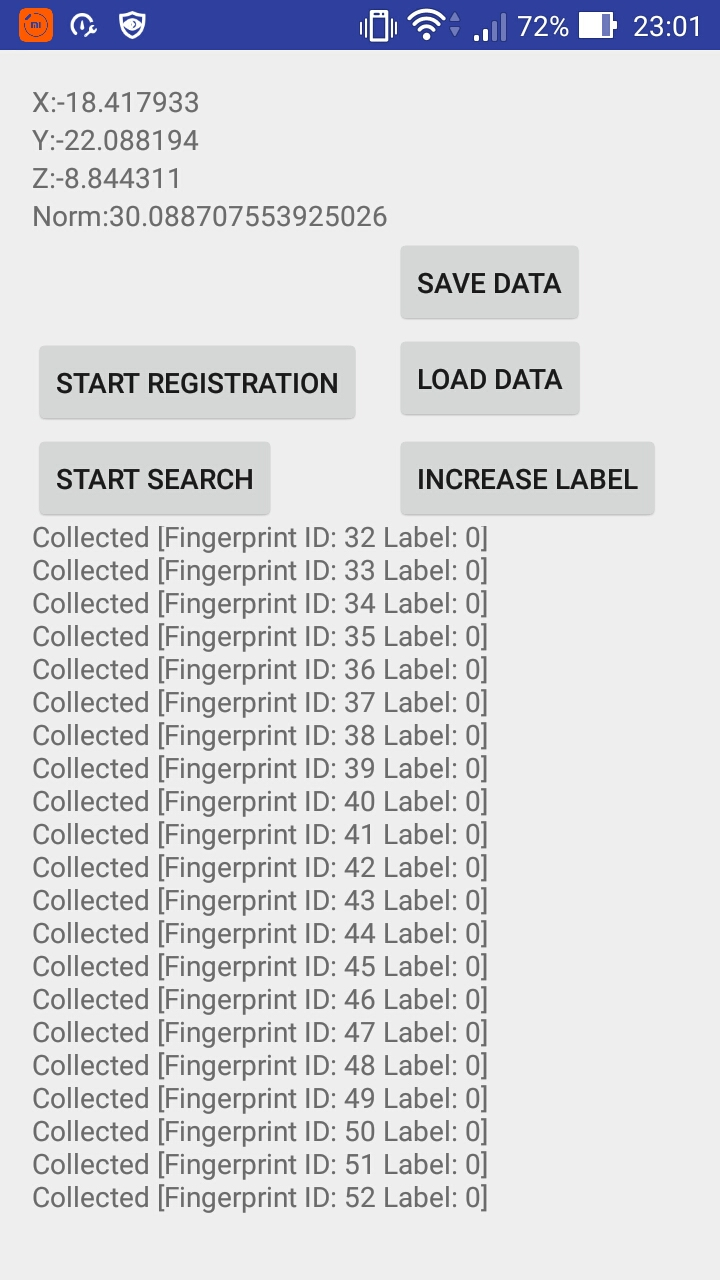
\includegraphics[width=0.3\linewidth]{img/app1} \,\,\,		
	     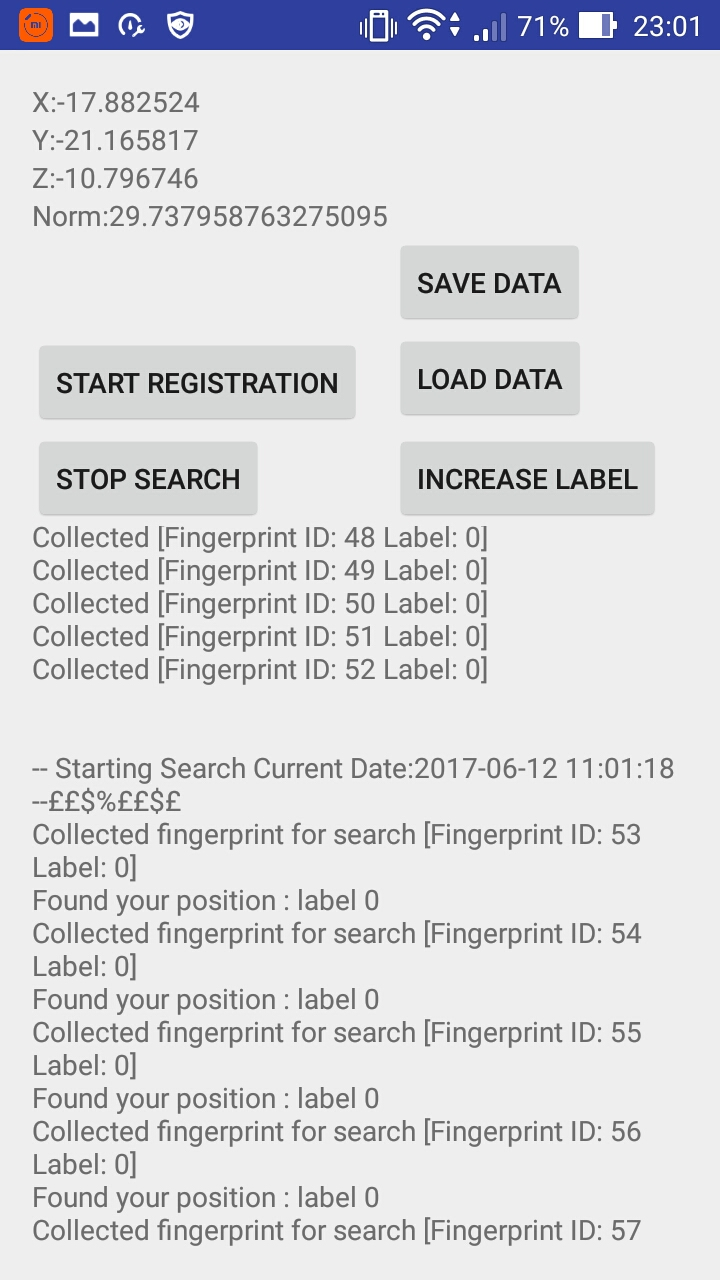
\includegraphics[width=0.3\linewidth]{img/app2}
		\end{align*}
	\end{frame}
	\begin{frame}{Descrizione dell'applicazione in fasi}
		\begin{enumerate}
			\item Dichiarazione ed istanziazione di una sottoclasse dell'interfaccia \textit{SensorListener} la quale ha lo scopo di ricevere l'intensit\`a delle onde magnetiche lungo gli assi visti precedentemente.
			\item Superata una certa soglia di onde magnetiche ricevute, esse vengono incapsulate dentro una \textit{fingerprint}.
			\item Dopo che l'utente d\`a l'input di fermare la raccolta delle onde parte in automatico la fase di \textit{preprocessing} dei dati. Per ogni \textit{fingerprint} vengono estratte attributi di natura statistica e non viene effettuata una scalatura sui dati poich\`e provoca un decadimento dell'accuratezza significativa.
			\item Quando l'utente preme sul pulsante "$\textit{Start search}$" inizia la raccolta di una \textit{fingerprint} per classificarla in base ai dati raccolti nei punti 1-2. Il classificatore usato in questa fase \`e il knn per via della sua facilit\`a d'implementazione.
		\end{enumerate}
	\end{frame}
	\begin{frame}{UML e codice}
		\begin{center}
				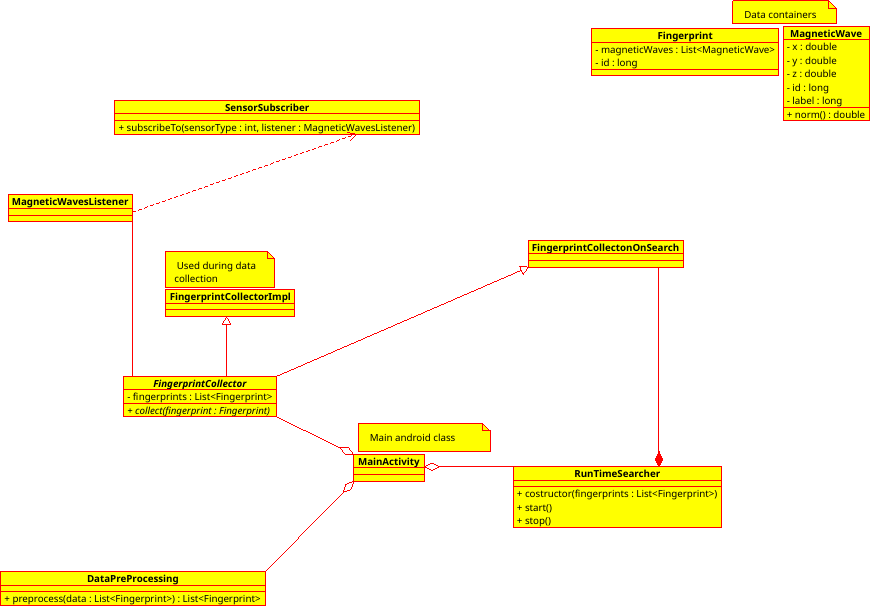
\includegraphics[width=1\linewidth]{img/class_diagram}
		\end{center}
	\end{frame}

	\begin{frame}{Linee di codice per file}
		\begin{center}
			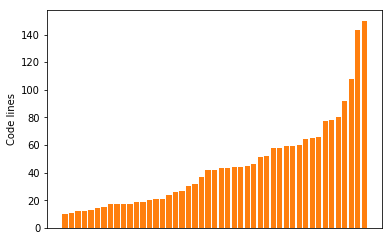
\includegraphics[width=1\linewidth]{img/codelines}
		\end{center}
	\end{frame}
	\begin{frame}{Librerie e linguaggi usati per i test}
		\begin{itemize}
			\item Nei test, per via delle ottime librerie votate all'analisi dei dati, \`e stato usato \textit{Python}
			\item Le librerie in questione sono \textit{NumPy, scikit-learn, Pandas, matplotlib}
		\end{itemize}
	\end{frame}
	\begin{frame}{Piano dei test}
		\begin{itemize}
			\item Raccolte circa 18000 onde magnetiche
			\item Metrica usata: errore sull'insieme di test $\left(1 - \dfrac{y_{true} = y_{pred}}{\lvert y\lvert } \right)$
			\item Qui sotto vediamo una piantina delle stanze scansionate con l'etichetta in sovrimpressione
		\end{itemize}
		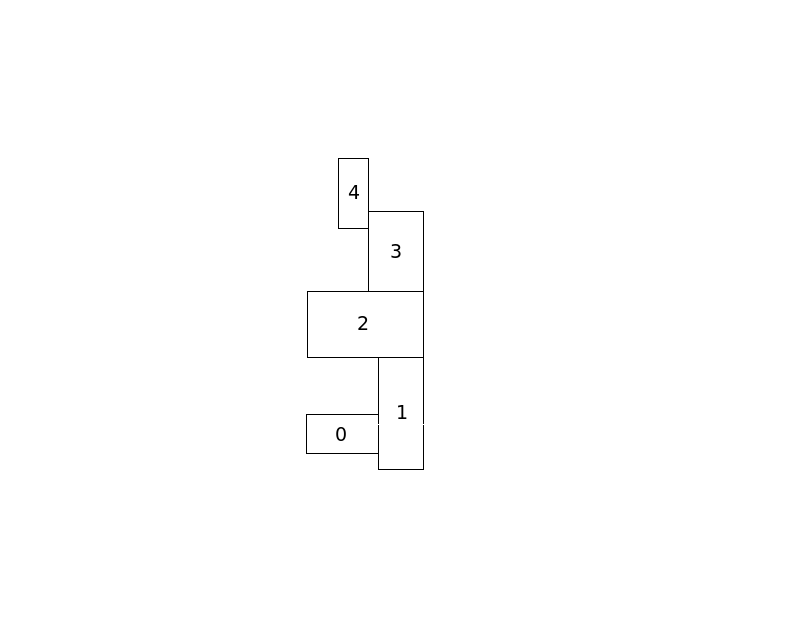
\includegraphics[width=0.7\linewidth]{img/test_pianta_casa}
	\end{frame}
	\begin{frame}{Analisi del rumore sui dati}
		\begin{itemize}
			\item Per analizzare il rumore sui dati mi sono posizionato fermo per 30 secondi registrando le onde magnetiche.
		\end{itemize}
		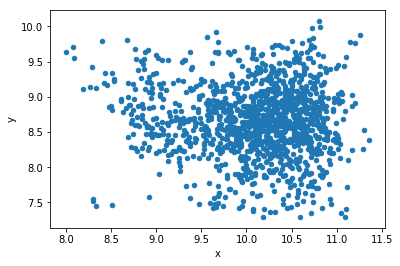
\includegraphics[width=0.7\linewidth]{img/xystand}
	\end{frame}
	\begin{frame}{Errore sui test dei classificatori}
		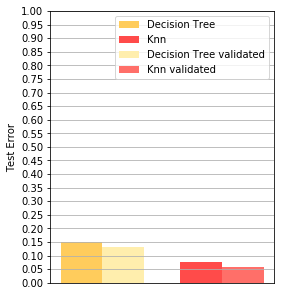
\includegraphics[width=0.7\linewidth]{img/test_error_classifiers}
	\end{frame}
	\begin{frame}{Errore sui test per etichetta}
		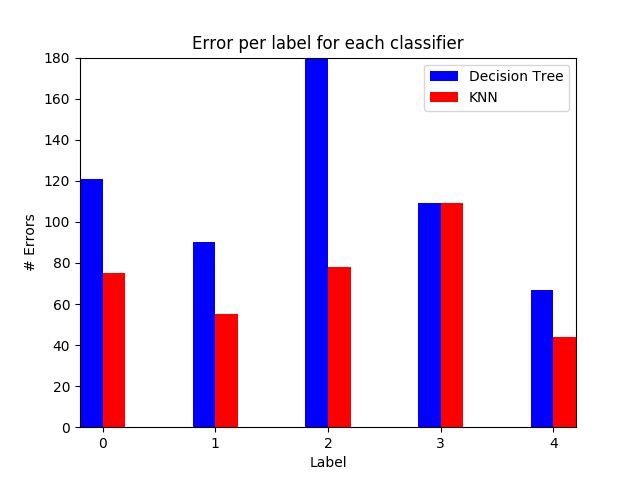
\includegraphics[width=1\linewidth]{img/test_error_per_label}
	\end{frame}
	\begin{frame}{Errore sui test per etichetta in percentuale}
		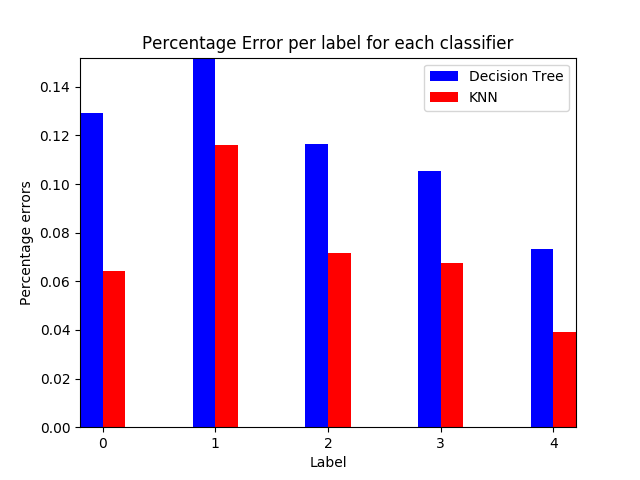
\includegraphics[width=1\linewidth]{img/test_error_per_label_percentage}
	\end{frame}
	\begin{frame}{Analisi del Knn al variare dell'iper-parametro k}
		\begin{center}
			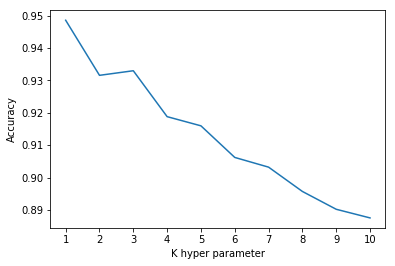
\includegraphics[width=1\linewidth]{img/accuracy_knn}
		\end{center}
	\end{frame}
	\begin{frame}{Analisi del Knn al variare dell'iper-parametro k}
		\begin{itemize}
			\item Se volessimo la massima accuratezza sceglieremmo k = 1 anche se sicuramente faremmo \textit{overfitting} sul modello
			\item Al contrario, scegliendo un k troppo alto otterremmo \textit{underfitting}
			\item L'esperienza con il modello aiuta molto nel scegliere gli intervalli di iper-parametri giusti da validare.
		\end{itemize}
	\end{frame}
	\begin{frame}{Analisi del Knn al variare dell'iper-parametro k}
		\begin{itemize}
			\item Un altro strumento per capire se ci stiamo adattando male ai dati sono le curve di validazione
		\end{itemize}
		\begin{figure}
			\centering
			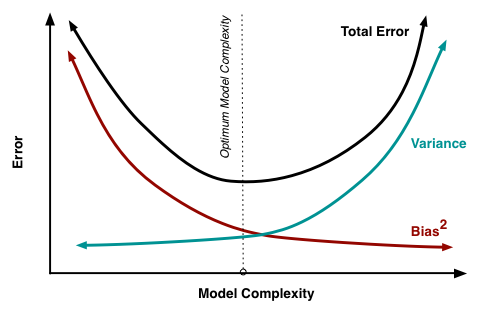
\includegraphics[width=0.7\linewidth]{img/biasvariance}
		\end{figure}
	\end{frame}
	\begin{frame}{Analisi del Knn al variare dell'iper-parametro k}
		\begin{itemize}
			\item L'errore complessivo del modello non \`e dato solo dalle predizioni sbagliate sull'insieme di test (\textit{bias}) ma anche dalla varianza, cio\`e che stiamo modellando anche il rumore generato dai dati.
			\item In generale nel knn all'aumentare di k diminuisce l'errore causato dalla varianza ma aumenta il \textit{bias}.
		\end{itemize}
	\end{frame}
	\begin{frame}{Analisi del Knn al variare dell'iper-parametro k}
		\begin{center}
			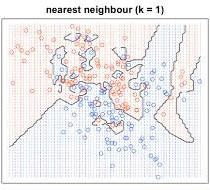
\includegraphics[width=0.8\linewidth]{img/1nn}
			%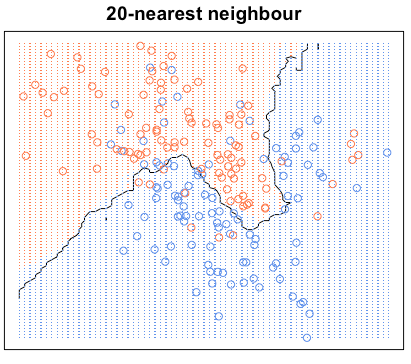
\includegraphics[width=1\linewidth]{img/20nearestneigh}
		\end{center}
	\end{frame}
	\begin{frame}{Analisi del Knn al variare dell'iper-parametro k}
		\begin{center}
		%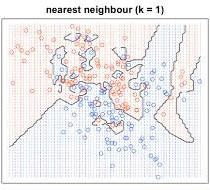
\includegraphics[width=1\linewidth]{img/1nn} \,\,\,
		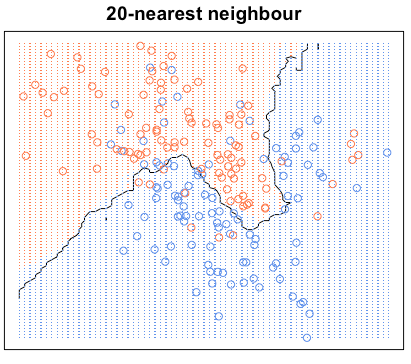
\includegraphics[width=0.8\linewidth]{img/20nearestneigh}
		\end{center}
	\end{frame}
	\begin{frame}{Analisi del Knn al variare dell'iper-parametro k}
		\begin{center}
			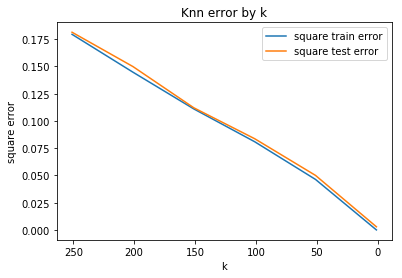
\includegraphics[width=1\linewidth]{img/biasvariance_knn}
		\end{center}
	\end{frame}
	\begin{frame}{Miglioramenti}
		\begin{itemize}
			\item Architettura client-server.
			\item Sfruttare altri sensori per identificare la posizione dell'utente.
			\item Sperimentare tecniche di estrazione e selezione di attributi e verificare come varia l'accuratezza.
			\item Provare altri classificatori pi\`u avanzati come svm o reti neurali
			\item Invece di usare un solo classificatore provare l'\textit{ensemble learning}
			\item Interfaccia grafica \textit{user-friendly}
		\end{itemize}
	\end{frame}
	\begin{frame}{Conclusioni}
		In conclusione abbiamo una base di applicazione \textit{Android} che raccoglie onde magnetiche dal magnetometro, le elabora e predice la posizione dei nuovi input tramite il \textit{knn}, un classificatore.
		Su computer sono stati effettuati test riguardanti  le onde magnetiche tramite l'esposizione di grafici. Abbiamo dimostrato che nei dati \`e presente rumore, per poi passare ad un confronto di accuratezza fra i classificatori presenti in cui ha ottenuto un minore errore sull'insieme di test il \textit{knn}. Ma \`e oro tutto ci\`o che luccica? Visti i buoni risultati, abbiamo approfondito  i risultati d'accuratezza al variare di k per scoprire di avere una funzione monotona decrescente. Abbiamo notato che se impostiamo un valore di k troppo basso incorriamo in \textit{overfitting} mentre in \textit{underfitting} se troppo alto.
	\end{frame}
\end{document}